\documentclass[10pt,letterpaper]{article}
\usepackage[utf8]{inputenc}

\title{CSE503 Performance Evaluation Study}
\author{Yitong Ding 446479 \& Qian Wu 425957}
\date{April 11, 2016}

\usepackage{graphicx}
\usepackage{xcolor}
\usepackage{listings}
\usepackage{float}
\usepackage{wrapfig}


\lstset{
    basicstyle=\scriptsize,
    extendedchars=false,
    numbers=left,
    frame=shadowbox,
    keywordstyle=\bf\color{blue},
    }



\begin{document}

\maketitle

\tableofcontents

\newpage



\section{Introduction}
There are many factors that result in the bottleneck of webpage performance, including poor database queries, network connections, which can be easily detected and analyzed through web development tools, such as Apache Bench. Apache Bench is a pre-installed tool for benchmarking the Apache HTTP server by sending a cluster of requests and recording time needed in response to various requests.  AB measures several aspects of the performance including concurrency, printing speed in HTML tables, performance under proxy server, etc. In this experiment, the stress test was performed under the concurrency parameter.

Similarly, the throughput of MongoDB database can be measured to evaluate the efficiency and performance of the database. In this experiment, two aspects of the database operations are measured: insertion and query, to cover reading and writing, the two basic processes that almost any other process involve.


\section{Experiment Platform}
We preformed our experiment on the Amazon EC2 instances. Amazon EC2 provides a diverse collection of instances that include a combination of different CPU, memory, storage, and networking capacity.These two experiments are performed with 6 different kinds of instances. All of them are general purpose – current generation instances, as the difference between them are usually small, making us easier to control the factors and do the comparison between them. The fact that we only choose 6 kinds of instance to run the benchmarks is because the difference between them are significant enough to show the impact of them on the performance of the web server. Besides, the price of AWS instance is also considered, as instance with 40 cores are much more ideal, but much more expensive. Besides, our application is relatively small, which means it might never needs such good server to hold. 

Here are the list of all the instances we used:
\begin{table}[h!]
\begin{center}
\begin{tabular}{| c || c | c | c | c |}
 \hline
 Name & vCPU & ECU & Memory (GiB) & Storage(GB)\\
 \hline
 t2.nano & 1 & Variable & 0.5 & EBS Only\\ 
 \hline
 t2.micro & 1 & Variable & 1 & EBS Only\\
 \hline
 t2.small & 1 & Variable & 2 & EBS Only\\ 
 \hline
 t2.medium & 2 & Variable & 4 & EBS Only\\
 \hline 
 t2.large & 2 & Variable & 8 & EBS Only\\
 \hline 
 m3.large & 2 & 6.5 & 7.5 & EBS Only\\
 \hline
\end{tabular}
\caption {AWS Instances Configuration}
\end{center}
\end{table}

The instances are chosen to cater the need of measuring the impact of one parameter on the performance while controlling the two other parameters. For instance, the comparison between t2.micro and t2.small would measure the effect of expansion of memory, the m3.medium instance is used to test the difference between EBS only storage and SSD storage, and the t2.nano instance is designed to test the performance with the limitation of small memory space (0.5GiB).

On the system side, we performed the experiment on the latest Amazon Linux AMI (version 2016.03.0 (HVM)), with kernel version 4.4.5. 

As for Amazon Linux AMI is based on Red Hat, the PHP we get from ‘yum’ is 5.3.29, which is not the latest version. But, since our application may not need to unitize the full performance of the server, the version of PHP shouldn’t matter that much.

The MongoDB version we used is  MongoDB Community Edition 3.2, which is the latest version. 

What’s more, as for the benchmarks we used is Python based, the Python version 2.7.10, and gcc with version 4.8.3. 


\section{Apache Performance Evaluation}
Running ApacheBench on AWS instances:

For each instance, the stress test is performed with 1000 requests, 10 or 100 at a time:

\begin{lstlisting}
ab -c 10 –n 1000 http://172.31.32.171/
ab -c 100 –n 1000 http://172.31.32.171/
\end{lstlisting}

Where –c denotes the number of concurrency and -n denotes the number of total requests, followed by the private IP address on the instance. The following output is obtained:
	
	\begin{figure}[!h]
	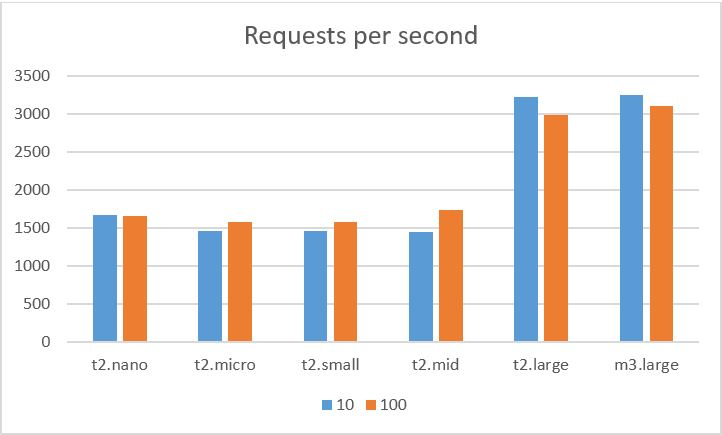
\includegraphics[width=0.7\textwidth]{ab_rs.jpg}
	\centering
	\caption{Apatch Requests per second}
	\end{figure}
	
	Of these parameters we focus on requests per second and the connection times, in which the 'processing' time is the most important matric for it measures the time between the sending and receiving the first byte of response. Because the concurrency is a factor that has presumably large impact on the processing efficiency, a comparison is made between a concurrency between 10 and 100. It is observed that there is roughly a 10 to 1 ratio between the concurrency of 100 and 10, so linear deterioration of performance is observed. 
	
	\begin{figure}[!h]
	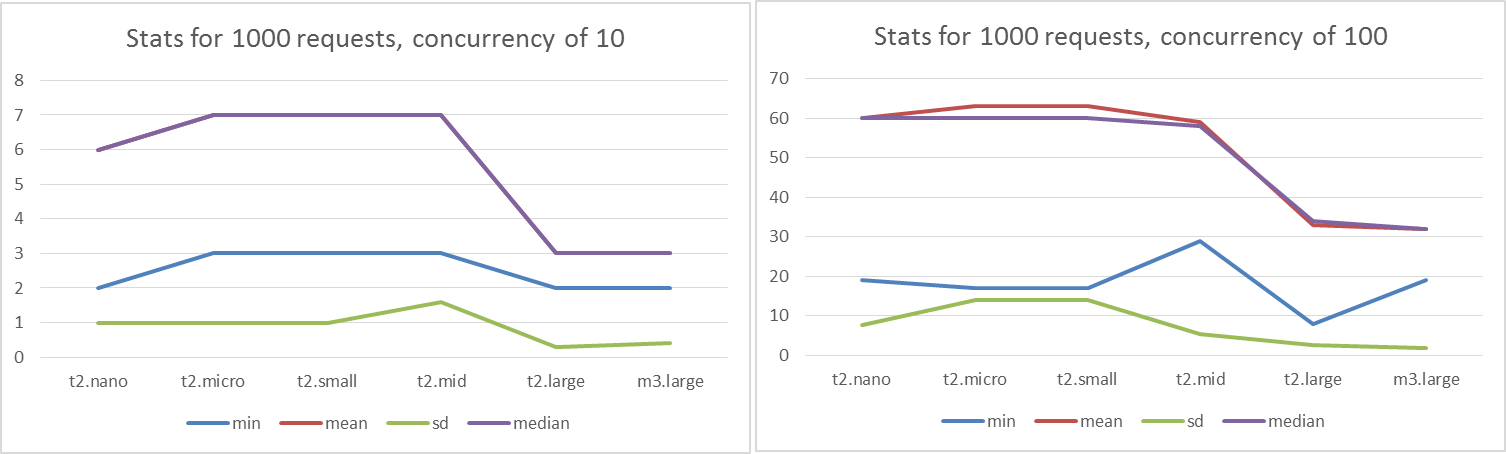
\includegraphics[width=\textwidth]{AB_result.png}
	\centering
	\caption{Apatch Connection Times}
	\end{figure}

We can see a huge boost when instance have a bigger RAM, as shown with t2.large and m3.large, who both have about 8 GiB of RAM. The boost is on requests per second as well as responds time. On the other hand, the number of CPU seems did not affect the Apatch performance by a lot.  

\section{MongoDB Performance Evaluation}
We used the Mongo-perf (not mongoperf) to do the evaluation on MongoDB. Mongo-perf is a micro benchmarking tool for the MongoDB server. It measures throughput of commands with regards to the number of threads. It is a python based benchmark, from whom we only use 2 test cases: simple insertion and simple query, to cover reading and writing from the database. We chose them as they are the most basic operation of the databases, and could be very representative. What’s more, inside the simple insertion and simple test scripts, there are actually a bunch of different test set ups. We would only use the empty insertion and empty query as the result would be affected by the content of the databases, and could represent the overall performance of the database. Another reason is that some of the test set up seems may case the database to crash and make the benchmark terminated with error. To avoid it, we decided to do the smallest scale test on the instances. Each of the test are set with threads of 1, 2, 4, 8 and 16 to test the performance of database under different pressure.

Here are the bench result: 

	\begin{figure}[!h]
	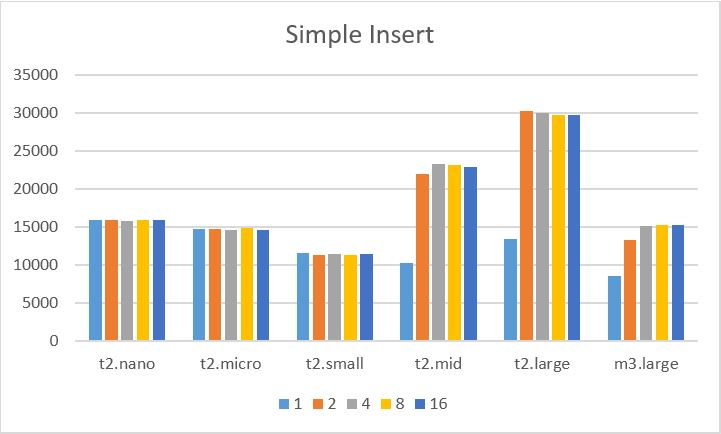
\includegraphics[width=0.7\textwidth]{mongo_insert.jpg}
	\centering
	\caption {MongoDB Insert Benchmark Result}
	\end{figure}
	
	\begin{figure}[!h]
	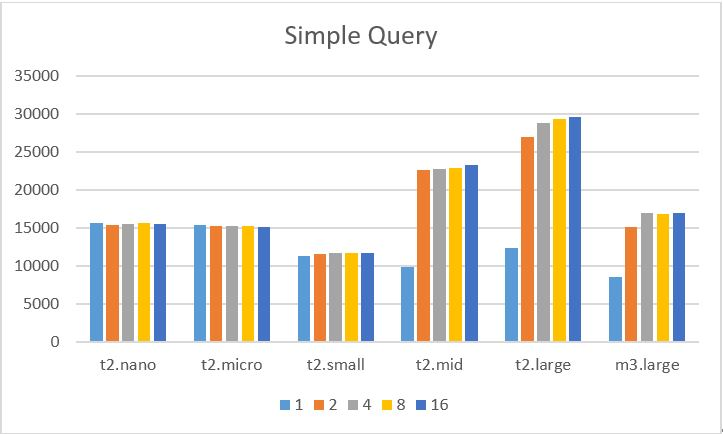
\includegraphics[width=0.7\textwidth]{mongo_query.jpg}
	\centering
	\caption {MongoDB Query Benchmark Result}
	\end{figure}
From the result, we can see that the CPU and RAM does impact the database performance a lot. 

For example, comparing the outcome of t2.small (with 1 vCPU \& 2 GiB RAM) and t2.mid (with 2 vCPU \& 4 GiB RAM), although the single thread performance is kind of the same, the multi-thread performance are boosted by twice.  It is reasonable since one more core means two thread can insert into the database simultaneously which result in twice performance.

Another example is shown between t2.mid (with 2 vCPU \& 4 GiB RAM) and t2.large (with 2 vCPU \& 8 GiB RAM). They both have 2 vCPUs, but one have RAM with as twice large as the other’s RAM. The performance boost by RAM is about 30\% on both single thread on multi-thread. The boost is not as significant as increasing the number of cores, but, still, it is quite a huge boost consider they both have only two virtual cores.

However, there are something out of our expectation. 

For the first one, the boost of RAM did not shown on the instance with one core, which are t2.nano, t2.micro and t2.small. This could cause by the CPU bottleneck effect as the only core they have are unable to fully utilize the RAM. However, there might be another reason, which is an interesting fact we found. The t2.nano and t2.micro instances were created on the ‘AWS Availability Zone’ - ‘us-west-2a’, and t2.small instance was created on ‘us-west-2c’. Could it means the performance of instance might be affect by the AWS zone it’s been hold? This might be tested to confirm in the future.

Secondly, the boost from using SSD as storage device did not boost the performance by huge amount as we expected. In fact, the performance decreases by a huge amount compare with t2.larege instance, where the only difference between them are the type of desk (assuming 8 and 7.5 GiB of RAM are the same). This could be caused by the fact that the SSD has only 32GB, which is too small to have a good performance, as we know the bigger the SSD is, the faster it can run. Besides, the AWS might use RAID as data storage, which is much faster if they choose RAID 0, 5 or 10. It is totally reasonable for AWS to do as it not only boost the date IO rate, but also make the clients’ data much more secure (as RAID data backup). This might also be tested to confirm in the future.

\section{Conclusion}
Hardware configuration of a server, with no doubt, has a huge impact on the performance of a server. More CPU and more RAM can always be good for a application, who can fully utilize them. As we shown in our work, the bottle neck of our application could be the RAM of our server, as the Apache performance is heavily impacted by the size of it. Database, somehow, would not affect the overall performance, as the read and writing rate are much higher than the request can be handle Apatch.

\end{document}
